\documentclass{beamer}\usepackage[]{graphicx}\usepackage[]{color}
% maxwidth is the original width if it is less than linewidth
% otherwise use linewidth (to make sure the graphics do not exceed the margin)
\makeatletter
\def\maxwidth{ %
  \ifdim\Gin@nat@width>\linewidth
    \linewidth
  \else
    \Gin@nat@width
  \fi
}
\makeatother

\definecolor{fgcolor}{rgb}{0.345, 0.345, 0.345}
\newcommand{\hlnum}[1]{\textcolor[rgb]{0.686,0.059,0.569}{#1}}%
\newcommand{\hlstr}[1]{\textcolor[rgb]{0.192,0.494,0.8}{#1}}%
\newcommand{\hlcom}[1]{\textcolor[rgb]{0.678,0.584,0.686}{\textit{#1}}}%
\newcommand{\hlopt}[1]{\textcolor[rgb]{0,0,0}{#1}}%
\newcommand{\hlstd}[1]{\textcolor[rgb]{0.345,0.345,0.345}{#1}}%
\newcommand{\hlkwa}[1]{\textcolor[rgb]{0.161,0.373,0.58}{\textbf{#1}}}%
\newcommand{\hlkwb}[1]{\textcolor[rgb]{0.69,0.353,0.396}{#1}}%
\newcommand{\hlkwc}[1]{\textcolor[rgb]{0.333,0.667,0.333}{#1}}%
\newcommand{\hlkwd}[1]{\textcolor[rgb]{0.737,0.353,0.396}{\textbf{#1}}}%
\let\hlipl\hlkwb

\usepackage{framed}
\makeatletter
\newenvironment{kframe}{%
 \def\at@end@of@kframe{}%
 \ifinner\ifhmode%
  \def\at@end@of@kframe{\end{minipage}}%
  \begin{minipage}{\columnwidth}%
 \fi\fi%
 \def\FrameCommand##1{\hskip\@totalleftmargin \hskip-\fboxsep
 \colorbox{shadecolor}{##1}\hskip-\fboxsep
     % There is no \\@totalrightmargin, so:
     \hskip-\linewidth \hskip-\@totalleftmargin \hskip\columnwidth}%
 \MakeFramed {\advance\hsize-\width
   \@totalleftmargin\z@ \linewidth\hsize
   \@setminipage}}%
 {\par\unskip\endMakeFramed%
 \at@end@of@kframe}
\makeatother

\definecolor{shadecolor}{rgb}{.97, .97, .97}
\definecolor{messagecolor}{rgb}{0, 0, 0}
\definecolor{warningcolor}{rgb}{1, 0, 1}
\definecolor{errorcolor}{rgb}{1, 0, 0}
\newenvironment{knitrout}{}{} % an empty environment to be redefined in TeX

\usepackage{alltt}
\usetheme{focus}
\definecolor{main}{RGB}{113, 93, 145}
\definecolor{background}{RGB}{248, 241, 255}
\usepackage[utf8]{inputenc}
\usepackage{polski}
\usepackage{amsfonts}
\usepackage{amsmath}
\usepackage{natbib}
\usepackage{graphicx}
\usepackage{array,booktabs,tabularx}
\usepackage{epstopdf}
\usepackage{colortbl, xcolor}
\usepackage{url}
\usepackage{ulem}
\usepackage{animate}

\newcommand\Fontvi{\fontsize{6}{7.2}\selectfont}

\newcommand{\btVFill}{\vskip0pt plus 1filll}

\title{HaDeX: an R package and \mbox{web-server} for analysis of \mbox{data} from HDX-MS experiments}
\date{}
\author{Dominik Cysewski}
\institute{Institute of Biochemistry and Biophysics \\ Polish Academy of Sciences}
\IfFileExists{upquote.sty}{\usepackage{upquote}}{}
\begin{document}




\maketitle

\begin{frame}{HDX-MS}

\begin{figure} 
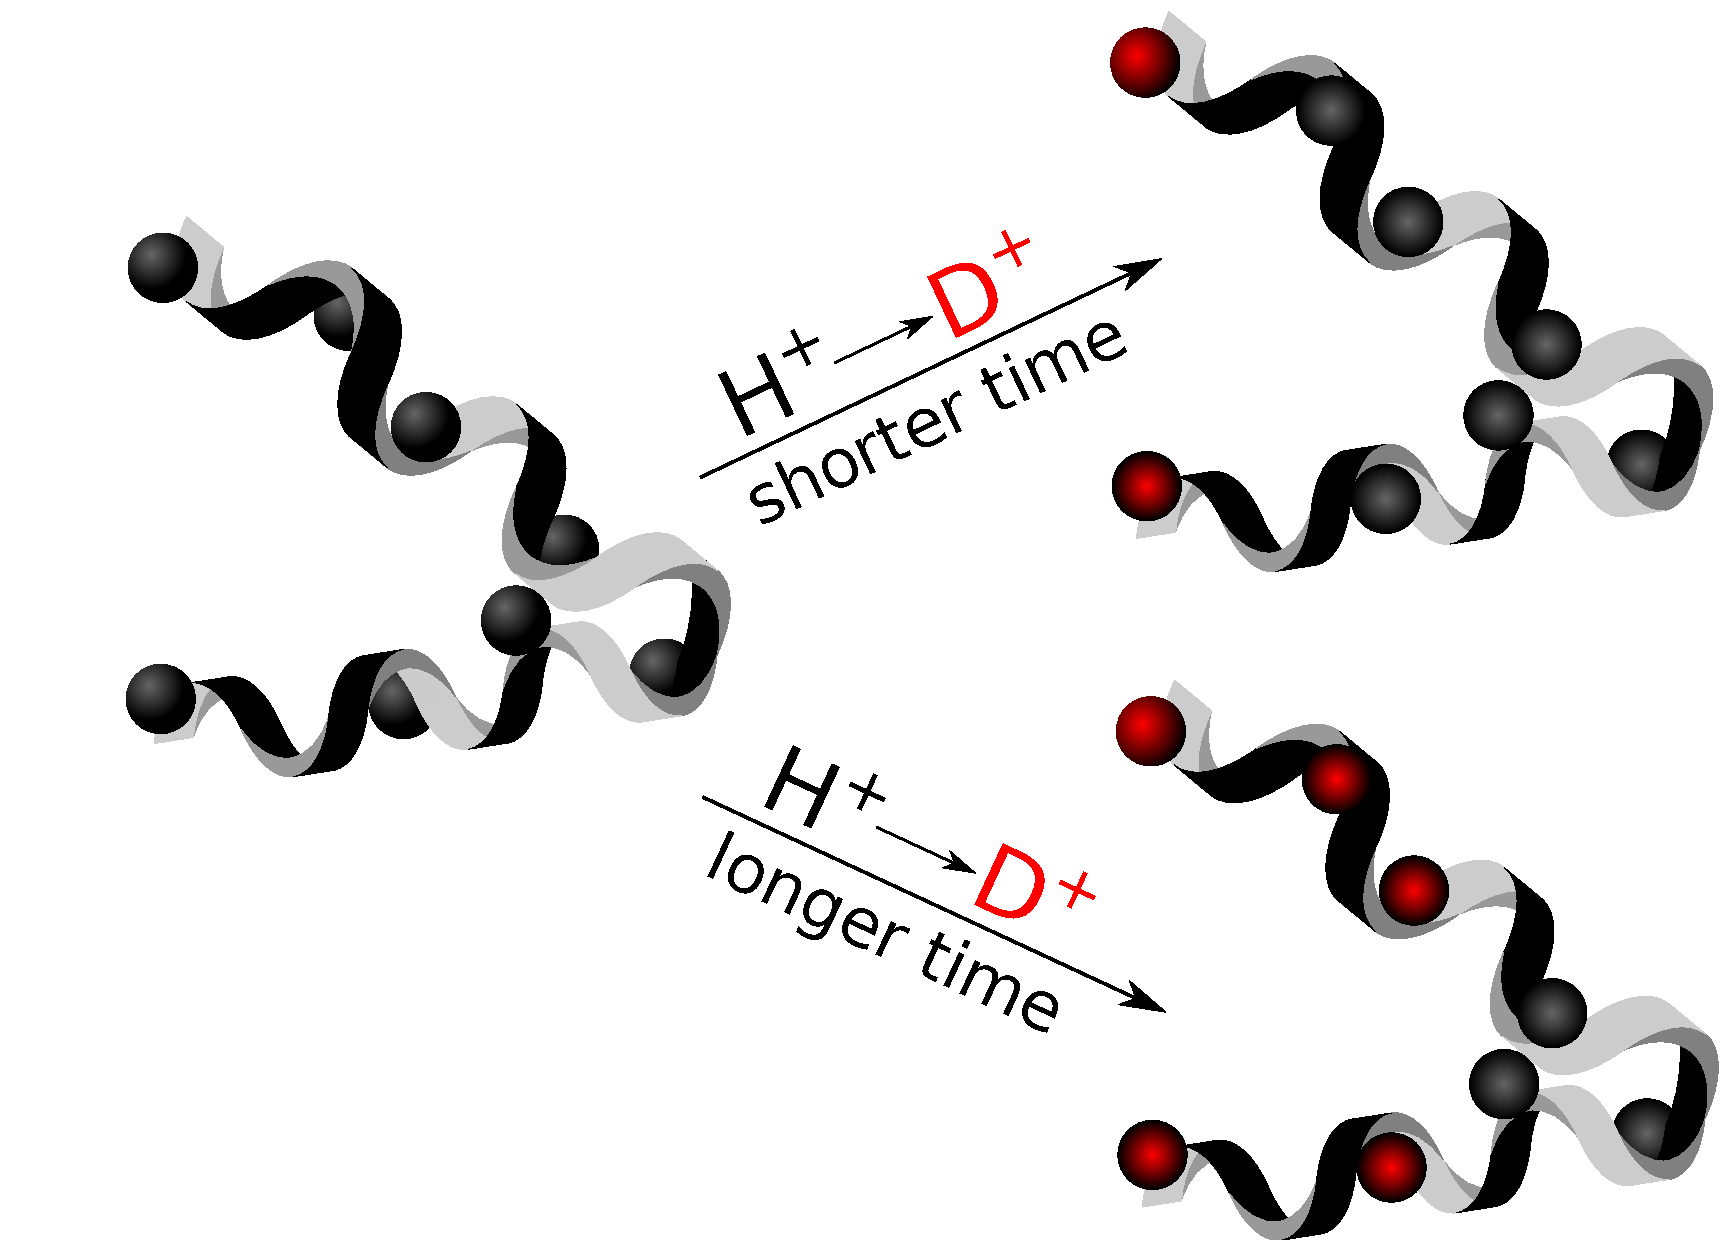
\includegraphics[width=0.80\textwidth]{static_figure/HDX-2.pdf}
\end{figure}

The longer incubation time, the more protected hydrogens are being replaced by deuters.

\end{frame}

\begin{frame}{Applications}

\begin{figure} 
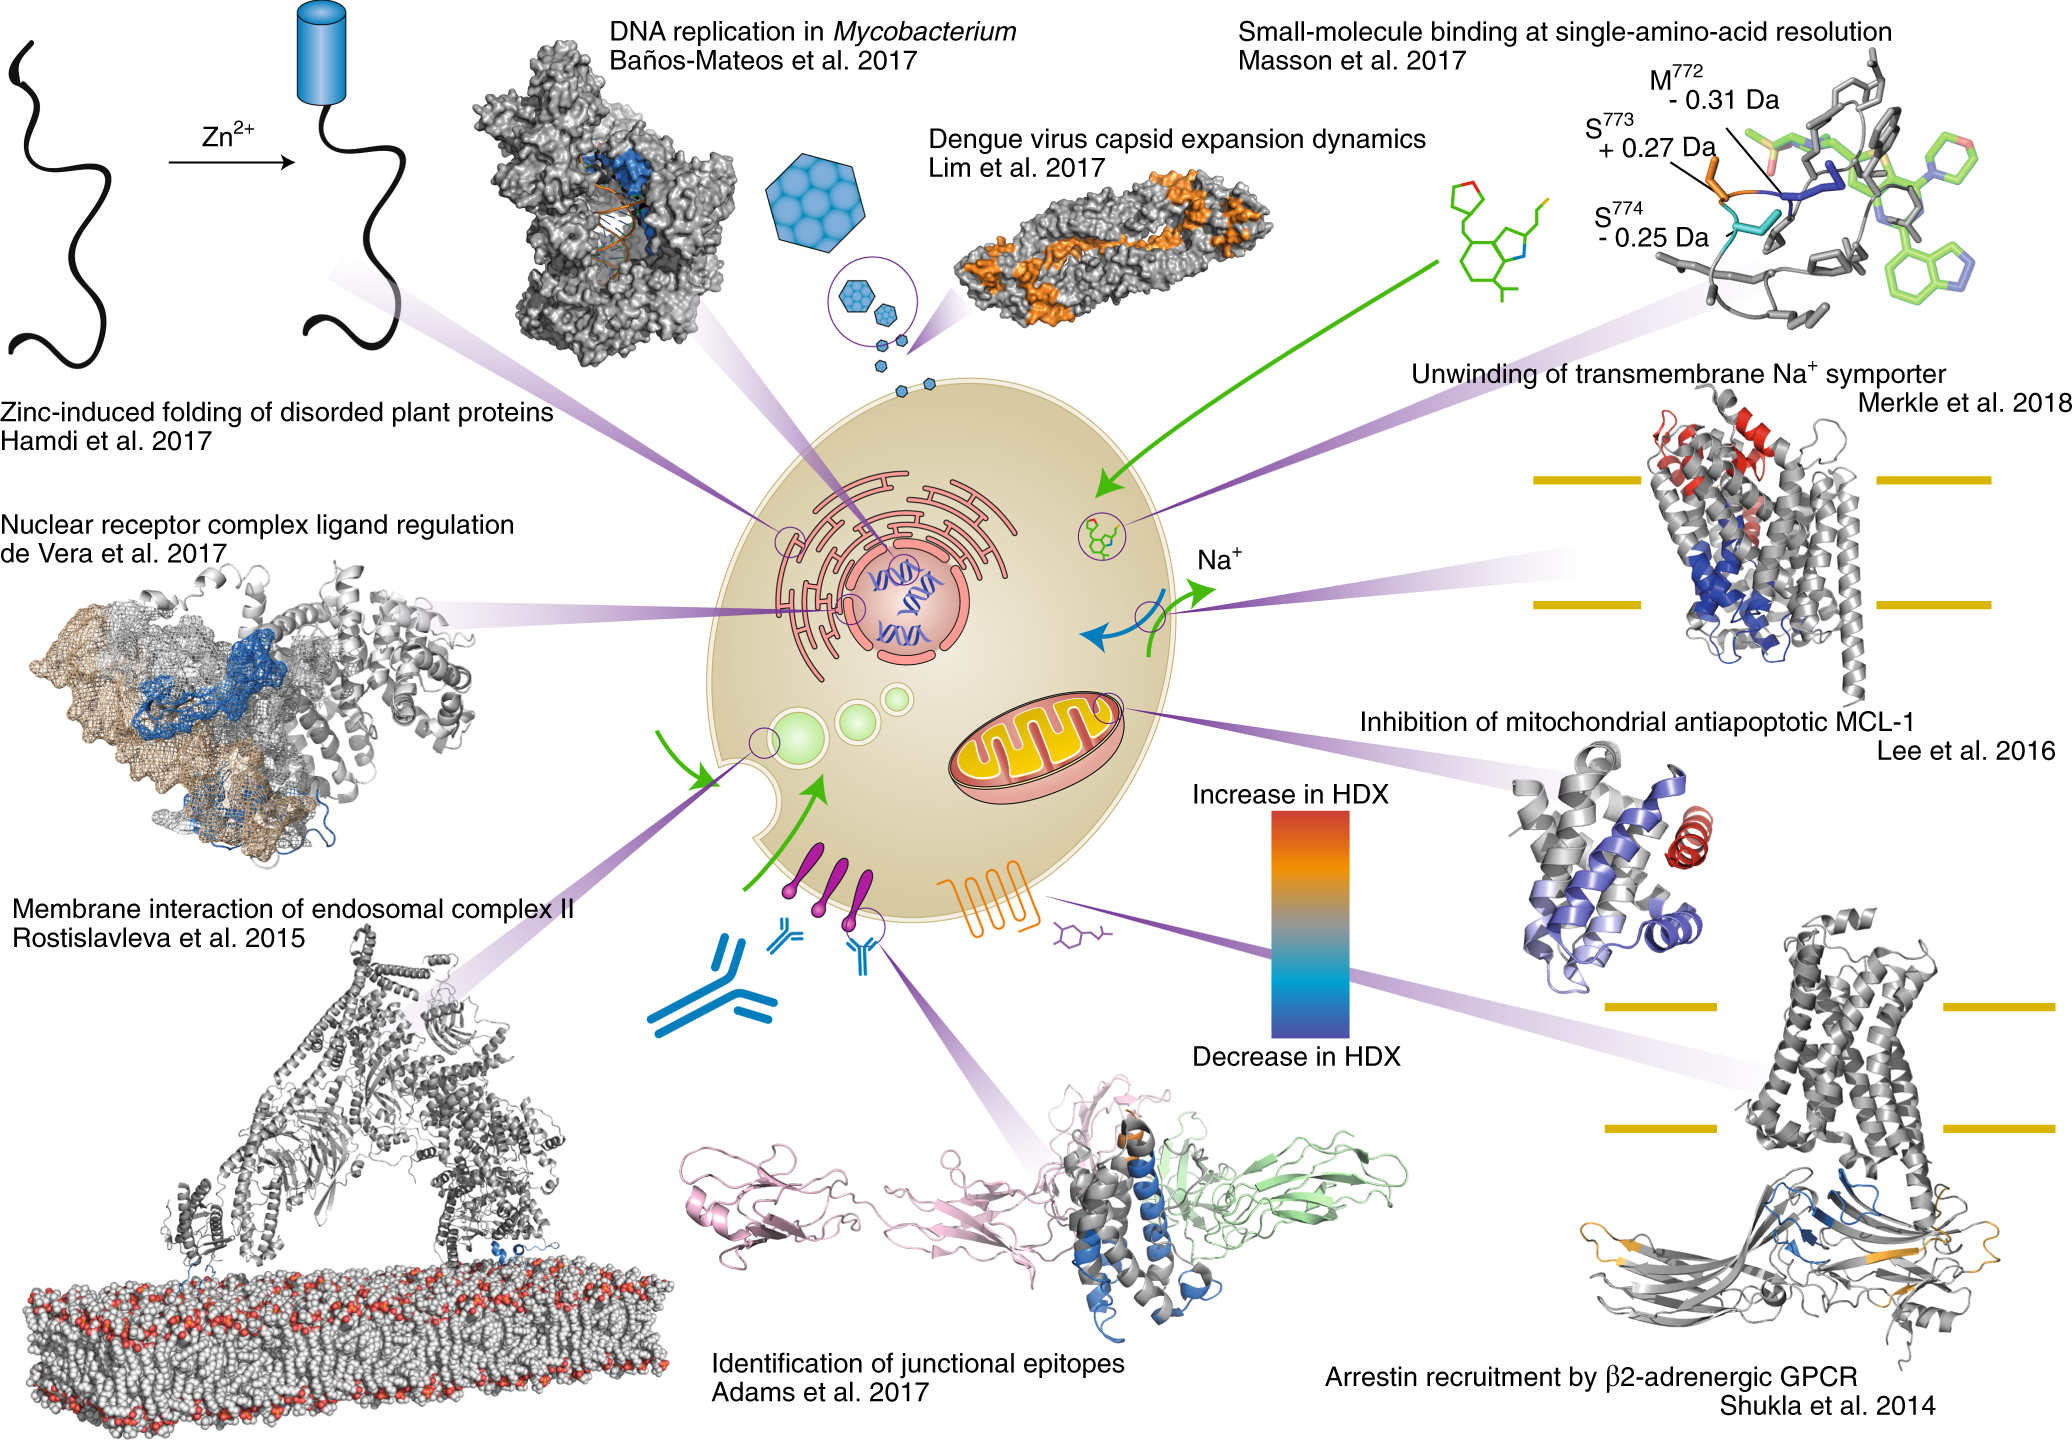
\includegraphics[width=0.85\textwidth]{static_figure/hdx-applications.png}
\end{figure}


\tiny G. R. Masson et. al. (2019).
Recommendations for performing, interpreting and reporting
hydrogen deuterium exchange mass spectrometry (HDX-MS)
experiments. Nature Methods, 16(7):595–602..

\end{frame}

\begin{frame}{Multi-state analysis}

\begin{knitrout}
\definecolor{shadecolor}{rgb}{0.969, 0.969, 0.969}\color{fgcolor}
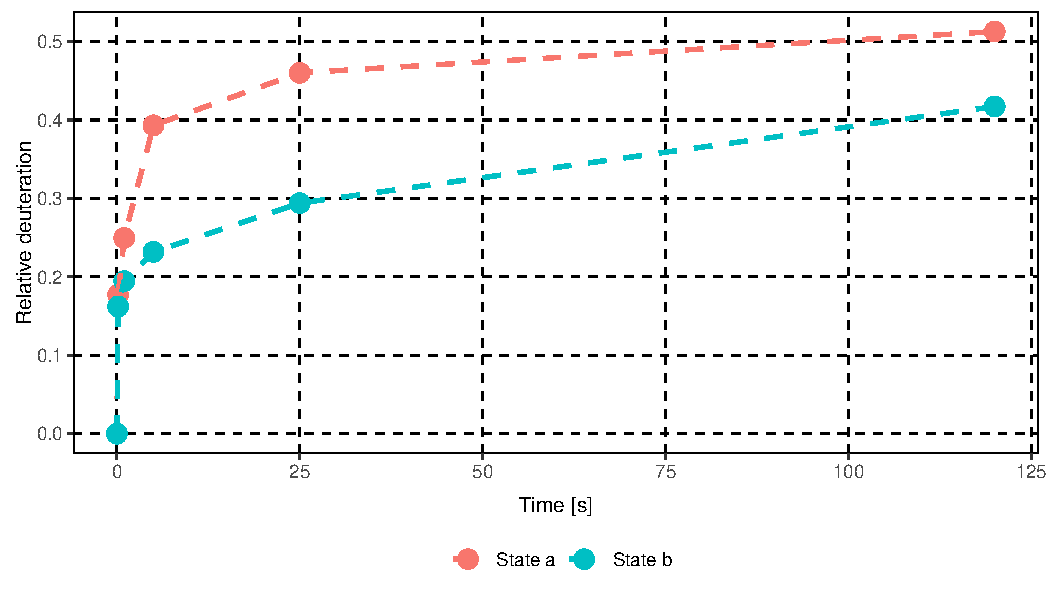
\includegraphics[width=\maxwidth]{figure/unnamed-chunk-1-1} 

\end{knitrout}


Peptides may come from proteins in differents states, i.e. bounded by different cofactors.

\end{frame}


\begin{frame}

\begin{center}
  \animategraphics[autoplay,loop,width=0.65\linewidth]{15}{static_figure/animation/gganim_plot}{0001}{0100}
\end{center}

During the analysis of the HDX-MS data we have to consider both time of the incubation and position of a peptide in a sequence. 
\end{frame}


\begin{frame}{Relative deuteration}
\begin{figure} 
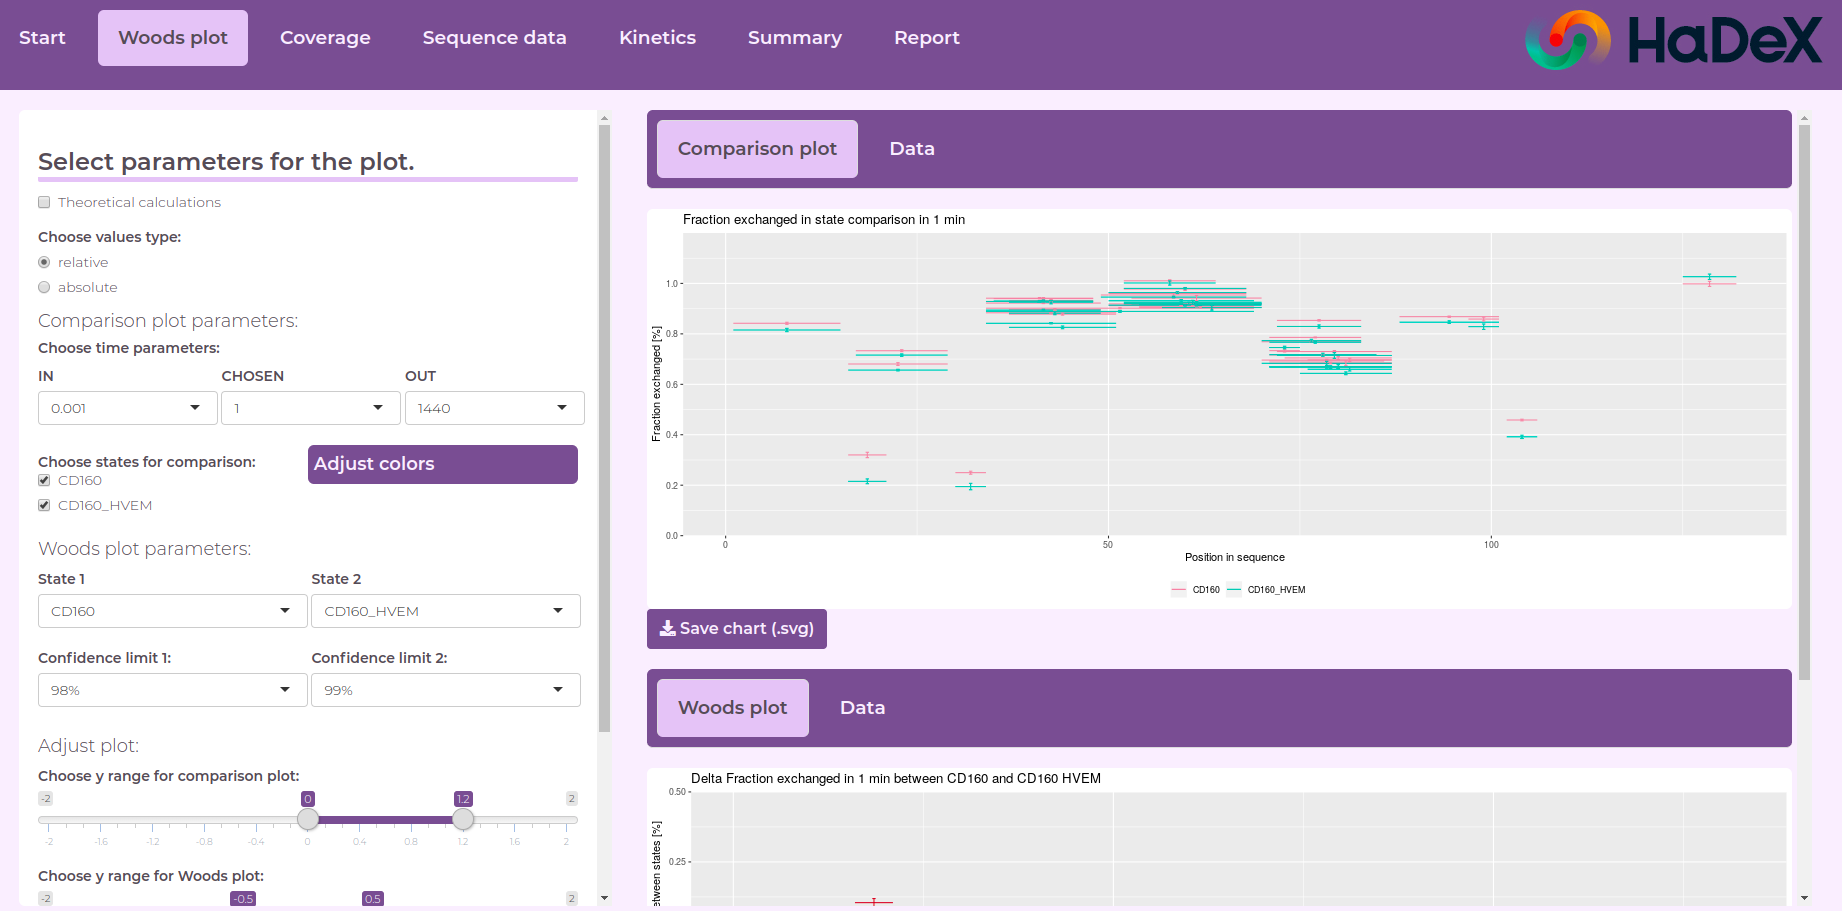
\includegraphics[width=\textwidth]{static_figure/HaDeX-2.png}
\end{figure}
\end{frame}

% \begin{frame}{Peptide coverage}
% \begin{figure} 
% 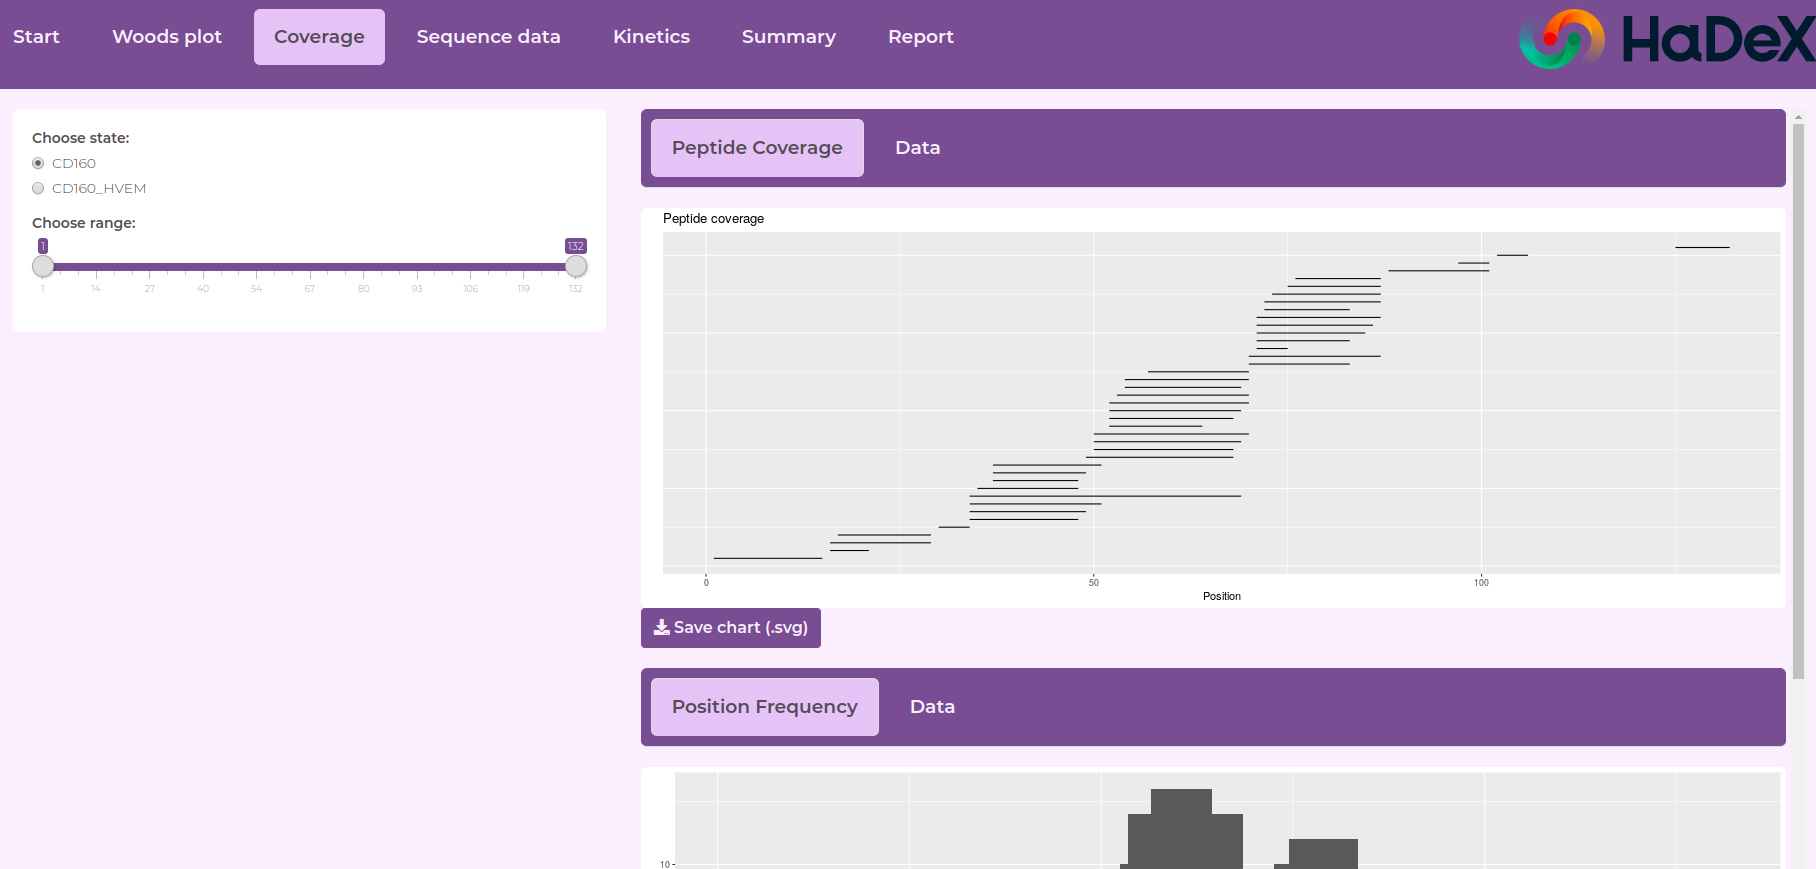
\includegraphics[width=\textwidth]{static_figure/HaDeX-4.png}
% \end{figure}
% \end{frame}


\begin{frame}{Deuteration kinetics}
\begin{figure} 
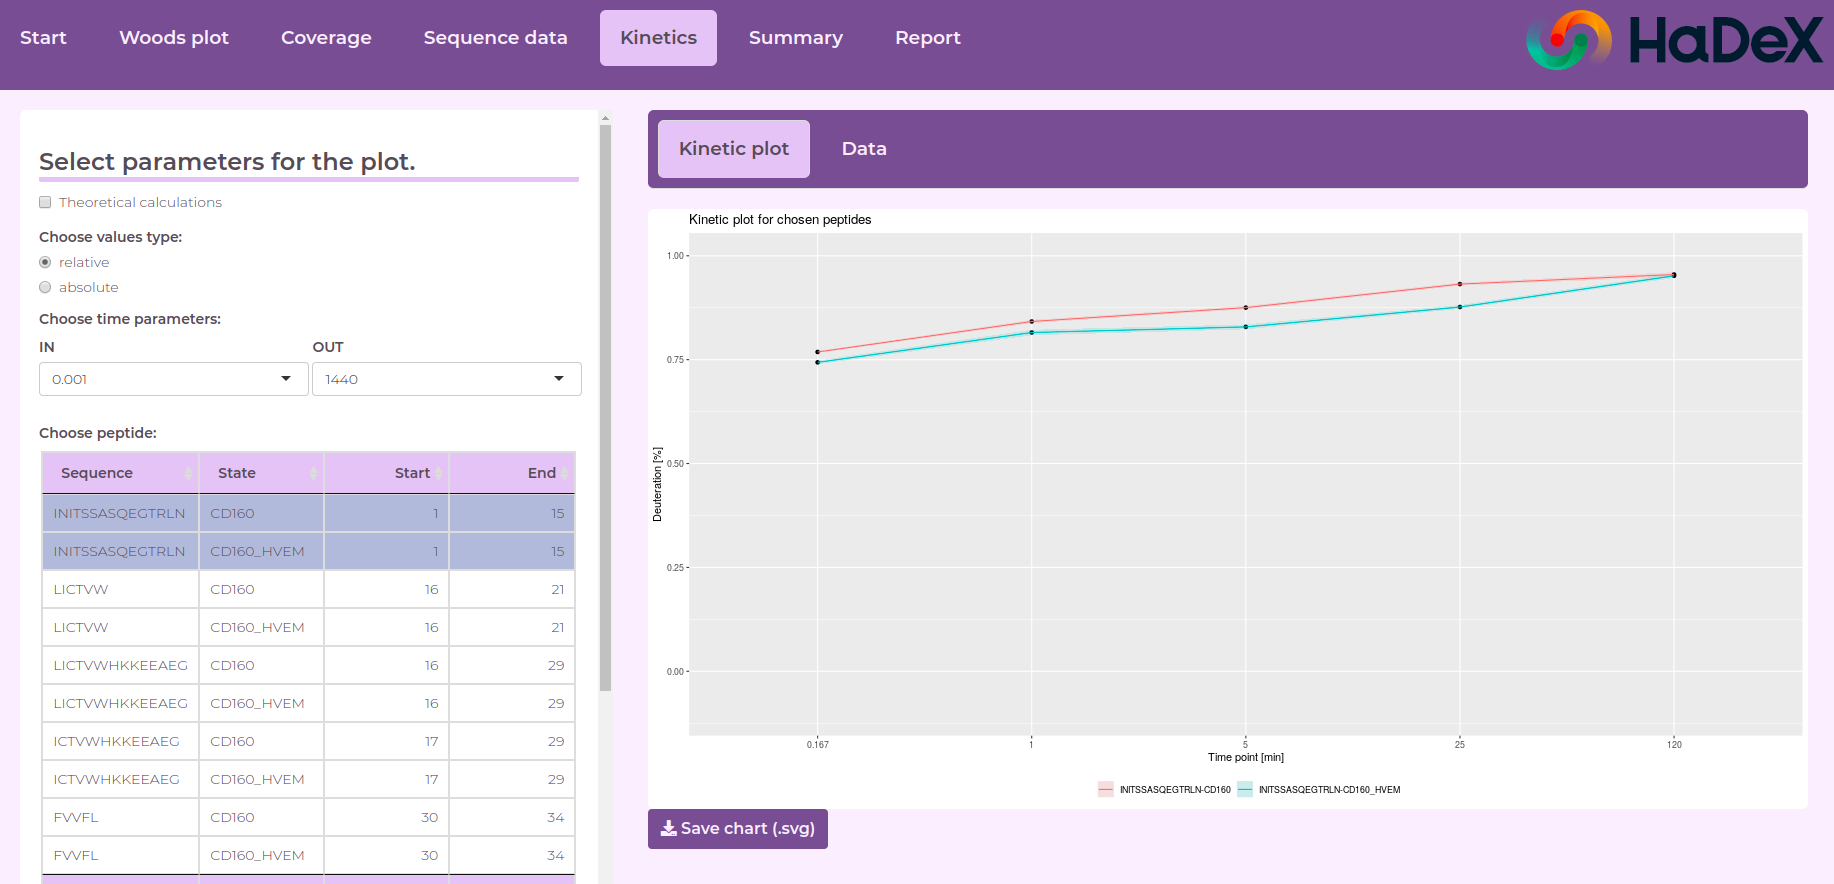
\includegraphics[width=\textwidth]{static_figure/HaDeX-6.png}
\end{figure}
\end{frame}


\begin{frame}{Reporting}
\begin{figure} 
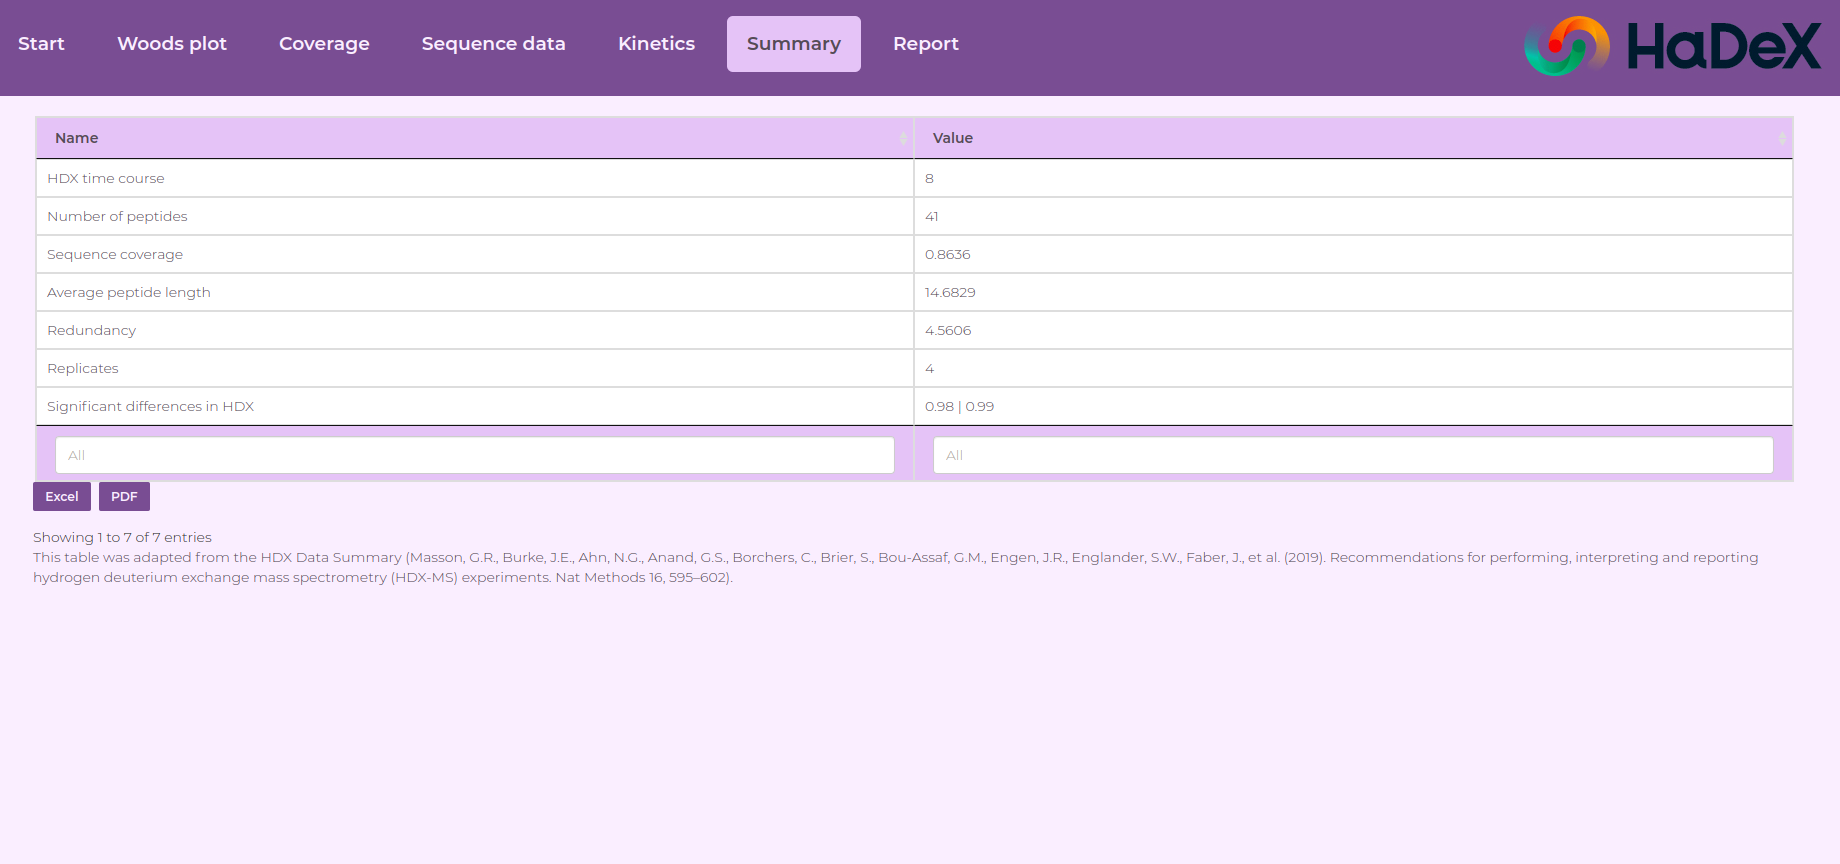
\includegraphics[width=0.8\textwidth]{static_figure/HaDeX-7.png}
\end{figure}

\begin{figure} 
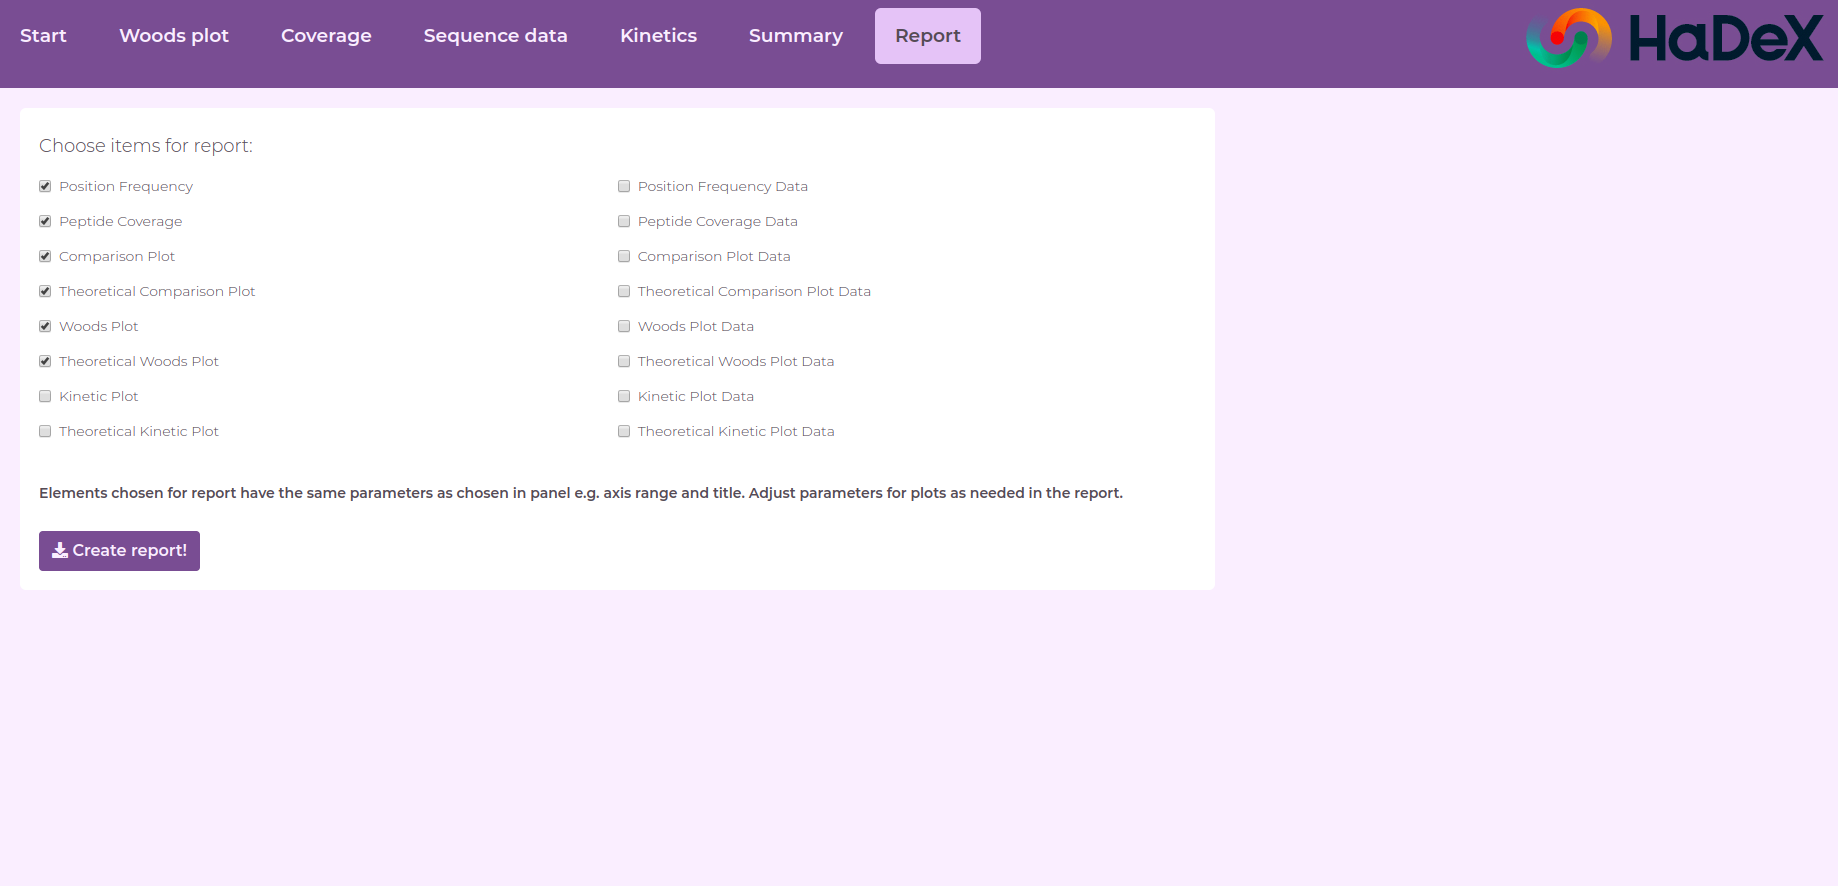
\includegraphics[width=0.8\textwidth]{static_figure/HaDeX-8.png}
\end{figure}
\end{frame}

\begin{frame}{Summary and availability}

Summary:

\begin{itemize}
\item rapidly developing technologies require a flexible framework,
\item the methods of data analysis should follow the development of both technology and expectations of its users.
\end{itemize}

\medskip

Availability:

\begin{itemize}
\item a web-server (\url{http://mslab-ibb.pl/shiny/HaDeX/}), 
\item the R package (\url{https://CRAN.R-project.org/package=HaDeX}),
\item a standalone software (\url{https://sourceforge.net/projects/HaDeX/}).
\end{itemize}
\end{frame} 



\begin{frame}{Acknowledgements}


\begin{columns}
\begin{column}{0.5\textwidth}
   \begin{itemize}
   \item Mass Spectrometry Lab, Institute of Biochemistry and Biophysics, PAS.
   \item MI$^2$ Data Lab, Faculty of Mathematics and Information Science, Warsaw University of Technology.
   \end{itemize}
\end{column}
\begin{column}{0.5\textwidth}  %%<--- here
    \begin{center}
    
\includegraphics[width=0.9\textwidth]{static_figure/ibb_logo.png}
     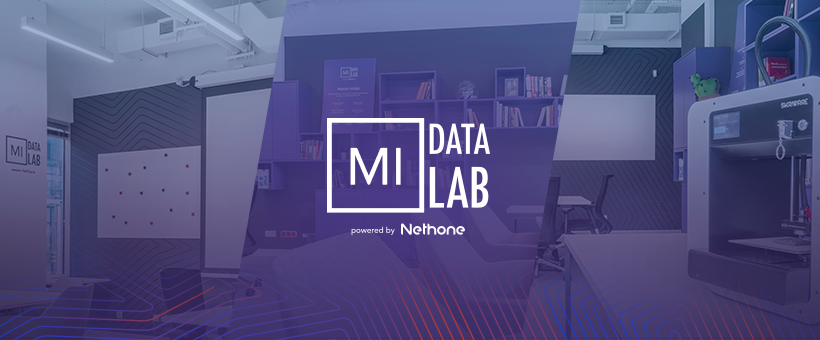
\includegraphics[width=0.9\textwidth]{static_figure/mi2.png}
     \end{center}
\end{column}
\end{columns}

\medskip 

\small Funding: Foundation of Polish Science TEAM TECH CORE FACILITY/2016-2/2 Mass Spectrometry of Biopharmaceuticals - improved methodologies for qualitative, quantitative and structural characterization of drugs, proteinaceous drug targets and diagnostic molecules.

\end{frame}

\begin{frame}{Acknowledgements}

\begin{columns}
\begin{column}{0.4\textwidth}
HaDeX developers:
  \begin{itemize}
    \item Weronika Puchala (main developer),
    \item Dominik Rafacz (frontend developer),
    \item Michał Burdukiewicz.
  \end{itemize}
\end{column}
\begin{column}{0.6\textwidth}  %%<--- here
  \begin{center}
    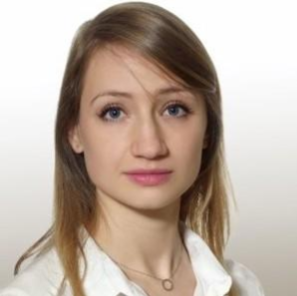
\includegraphics[width=0.35\textwidth]{static_figure/weronika.png}
    \\
    
\includegraphics[width=0.35\textwidth]{static_figure/dominik.png}
    \\
    
\includegraphics[width=0.35\textwidth,height=0.35\textwidth]{static_figure/michal.jpg}
  \end{center}
\end{column}
\end{columns}
\end{frame} 

\end{document}
